\chapter{System Software}
\label{chap:system_software}
Having discussed how the functionality of each subsystem is implemented in chapter \ref{chap:hardware_subsystems} we now provide a description of the software that brings these subsystems together into a complete system. 


\section{Monitoring Device}
For the reasons discussed in section \ref{sec:design_challenges}, the functionality of the monitoring device is kept simple and can be summarized as gathering data from the sensors, storing the data offline in the SD card when the ZigBee wireless connection is not available, and sending the gathered data to the base station. Figure \ref{fig:dataflow_monitoring_device} illustrates the data flow on the monitoring device.

\begin{figure}
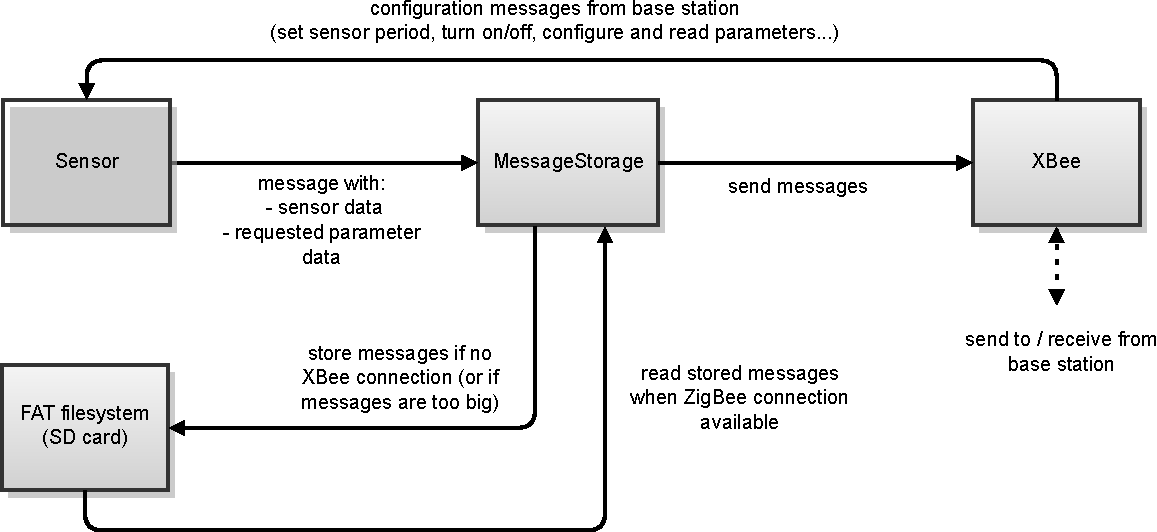
\includegraphics[width=\textwidth]{Images/monitoringdevice_dataflow}
\caption{Monitoring Device: dataflow}
\label{fig:dataflow_monitoring_device}
\end{figure}

Furthermore, to keep the energy efficiency focus, this data flow has to be implemented using periodic sampling and automated data acquisition whenever possible. The following subsections will describe these implementation details for the system software on the monitoring device.

\subsection{Development Paradigm and Environment}
The monitoring device software was developed using a mix of C++ and C, with IAR Embedded Workshop for ARM as the development environment. Using this mix of object-oriented and procedural programming paradigms, we aimed to achieve the best of both worlds - C++ classes were created to take advantage of polymorphism and encapsulation where possible, while pure C was used in places where small and efficient functions (e.g for handling DMA callbacks or audio-related tasks) were needed.

The choice of object-oriented paradigm (OOP) and C++ may be considered unusual for a highly integrated embedded system, but we considered the advantages to outweigh the penalties for our project. The 128 KB of RAM is enough to compensate for overheads introduced by C++, and sensor drivers involve handling tightly coupled data and functionality, which is suitable for modelling them as objects. Additionally, deriving all sensor implementations from the same Sensor base class allowed the integration of sensors into the final system in a plug-and-play manner, since they all share the same interface.



\subsection{Low Energy Periodic Sampling, Sensor Interface and Drivers}
\begin{figure}
\centering
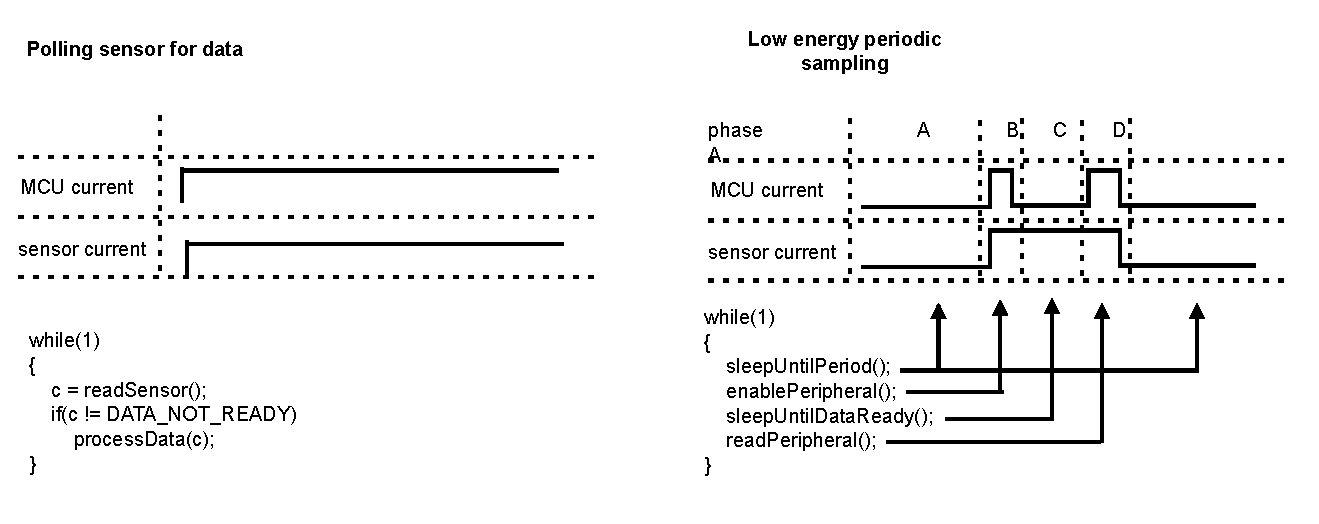
\includegraphics[width=\textwidth]{Images/sampling_comparison}
\caption{Sampling comparison}
\label{fig:sampling_comparison}
\end{figure}
We now discuss our definition of low energy periodic sampling for the monitoring device, and the relevant OOP basis we constructed towards its implementation. The basic idea behind low energy periodic sampling is that a receiving a continuous stream of data from all the sensors all the time is not necessary for monitoring purposes is unnecessary. Depending on the sensor type, receiving a sample with a period of tens of seconds, perhaps minutes can be sufficient for analysis. In this case, since the sensor and the microcontroller are not required to be active all the time, significant energy savings can be achieved by putting them into sleep mode until the start of the next period. This scheme can be further extended by introducing an additional period of sleep for the microcontroller after it awakens the sensor and waits for data. An illustration of how this compares with the continuous polling approach can be found in figure \ref{fig:sampling_comparison}, with a more detailed explanation of the power management phases in table \ref{tab:power_phases}. It can be seen that the low energy periodic sampling offers much less current consumption compared to polling.

\begin{table}
\centering
\begin{tabular}{|l|m{1.5cm}|m{1.5cm}|m{2.5cm}|m{4.5cm}|}
\hline
	\textbf{Phase}  &
	\textbf{MCU state}  &
	\bfseries Sensor state  &
	\textbf{Duration}  &
	\textbf{Description}  \\ 
\hline
	Phase A &
	asleep  &
	asleep  &
	as desired  &
	both sleepig and waiting for next sampling period to start  \\ 
\hline
	Phase B &
	awake  &
	awake  &
	MCU dependent (wakeup time)  &
	microcontroller wakes up peripheral, peripheral starts sampling  \\ 
\hline
	Phase C &
	asleep  &
	awake  &
	sensor dependent (sampling rate)  &
	microcontroller sleeps while waiting for peripheral to complete sampling  \\ 
\hline
	Phase D &
	awake  &
	awake  &
	bus dependent (data read speed)  &
	data ready, microcontroller reads data from peripheral, then go back to Phase A   \\ 
\hline 
\end{tabular}
\caption{Periodic sampling power phases}
\label{tab:power_phases} 
\end{table}

This energy saving scheme can be applied to any sensor or peripheral that supports sleep mode. As we chose all only sleep-supporting sensors for our implementation, we were able to identify a set of properties and functions common to all sensors which forms the Sensor base class. The properties and methods defined in the class are listed in section \ref{list:sensor_interface}. 

To summarize, the \textit{setSleepState} function is used to put the sensor to sleep and wake it up, the \textit{sampleSensorData} acquires data from the sensor into internal buffers, and \textit{readSensorData} gives access to the data in the internal buffers wrapped in a \textit{SensorMessage} structure (described in section \ref{sec:message_types}). Individual sensors drivers are derived from this base class and implement the common methods in their specific way, as described in chapter \ref{chap:hardware_subsystems} 


\subsection{Timekeeping and Alarm System}
\label{sec:timekeeping}
Timekeeping and Alarms System
To implement the periodic sampling scheme discussed in the previous section, it is necessary to keep track of real time and trigger an alarm when an action (such as waking up the sensor from sleep) is needed. The same implementation can be used to provide small fixed-length blocking delays in code, which are useful in the driver implementations.

The EFM32 has a dedicated  Real Time Counter (RTC) peripheral which makes this implementation easy, but the challenge is once again doing this in an energy efficient way. For example, it is possible to configure a system tick that wakes up the MCU every millisecond and updates an internal counter, but waking up every millisecond is very inefficient in terms of energy. Most of the time, we require periodic alarms that are generated in the range of seconds for the low energy periodic sampling scheme. This means timer tick interrupts that wake up the processor every second is enough for our purposes.

To our convenience, the EFM32 RTC peripheral can be kept active down to deep sleep (mode EM2) by using the low frequency oscillator (\TODO{} refer to section TODO section:pcboscillators for details) and be configured to generate interrupts only when the tick counter reaches a certain value. This allows us to do timekeeping at a very low energy cost and generate alarms with second-precision. Additionally, it is still possible to generate millisecond-accurate interrupts using the secondary compare register when needed.

This functionality is encapsulated inside the \textit{AlarmManager} class, which offers easy energy-efficient timekeeping and periodic alarm generation functionality. It can be used to generate periodic or single-shot alarms that become triggered after a given number of internal ticks. The triggered alarm executes a callback function specified at the alarm creation time. The internal tick period itself is configurable from milliseconds to hours. The class also supports an energy efficient delay function that can be used to create a blocking delay with millisecond resolution while putting the MCU to sleep in the desired mode. Finally, the class exposes the number of seconds and/or milliseconds elapsed since the start of monitoring device operation, which is used to generate timestamps for the sensor messages that are sent to the base station \TODO{:} connect this to appropriate section about relative timekeeping.

One final issue regarding timekeeping is persistence across reboots. The monitoring device may stop and restart execution after some time due to the battery running out. To keep the integrity of timestamps, the RTC second counter is regularly backed up to the SD card and re-read upon reboot.

\subsection{Task Scheduling and Sleep Management}
While it is intuitive to model the functionality that reads data from each sensor as a separate task and then use a real-time operating system to execute these tasks concurrently, we preferred not to use an RTOS as they typically use high-frequency system tick interrupts to do task scheduling and dispatching, and a high frequency system tick is not compliant with our low energy goals due to the reasons explained in the previous section. There are RTOS ports for EFM32 that avoid this, Therefore, we rely on the periodic alarms generated by the AlarmManager to trigger sensor readings.

The problem with this approach is the fact that the alarm handler callback functions are executed inside the interrupt context. If the alarm handler takes a long time to execute (for example, read a large amount of data from the sensor) this will result in staying in the interrupt context for a long time. Even though the EFM32 supports nested interrupts, it is considered to be bad practice to have big interrupt service routines since it can introduce instabilities into the system. Our solution to the problem was to adopt the deferred procedure call (DPC) approach for periodic readings. Illustrated in figure \ref{fig:deferred_reading} a DCP shifts the execution of time consuming data acquisition functions to the main context instead of doing them inside the interrupt context..

\begin{figure}[htb]
\centering
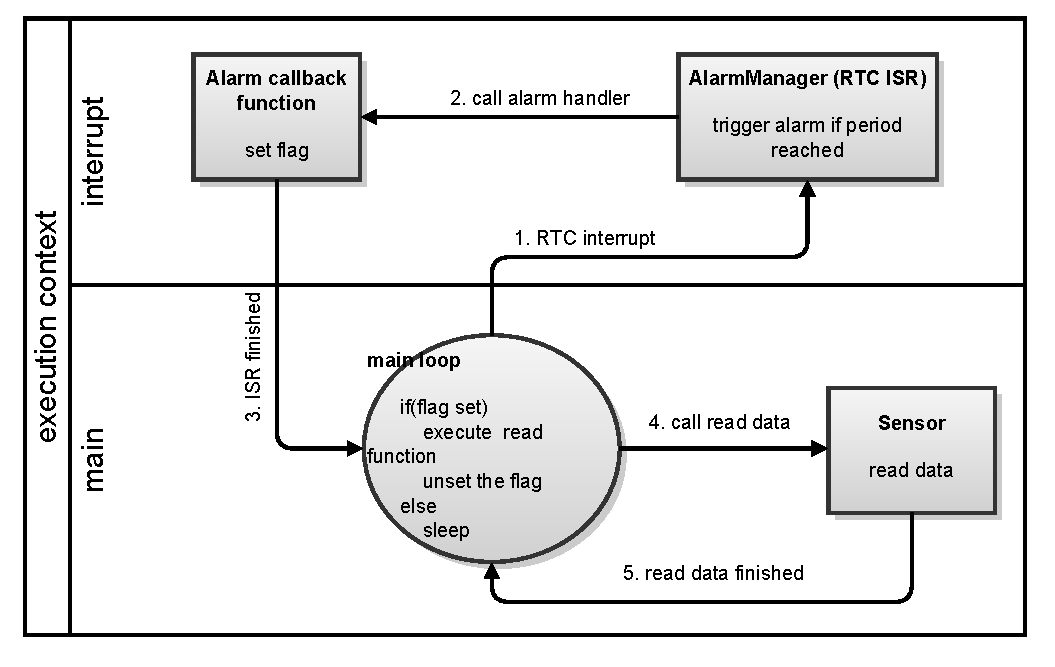
\includegraphics[width=\textwidth]{Images/deferred_reading}
\caption{Deferred reading}
\label{fig:deferred_reading}
\end{figure}

In this scheme, the interrupt handlers do not do any processing beyond taking actions so that received data is not lost but buffered in memory. The ISR then sets a flag indicating that the corresponding handler task should be executed. When the control returns to the execution loop, it checks each flag in order of decreasing task priority, executes the task if its flag is set and clears the flag afterwards. The processor then goes to sleep until the next interrupt.

Since the order of checking the task flags determine the execution priority and because the scheme is not preemptive, the tasks must be designed to be short (i.e not block execution for long periods). Not observing this principle can cause a big backlog of tasks to be executed and leave the processor no time to sleep.

A final consideration is the handling of asynchronous interrupts during sleep. This scheme is dependent on interrupts from hardware waking up the MCU from sleep, so care must be taken to ensure that the sleep level chosen will not disable the hardware that will generate the interrupts. 

\subsection {Message Storage System}
In order not to lose any acquired samples when the wireless connection to the base station is not available, it is necessary to save the samples on persistent storage. The project utilizes an SD card for this purpose, as described in section \ref{sec:data_storage}. This chapter focuses on the software component which abstracts the data storage for the convenience of sensor systems.

It is possible to model the message storage requirements of the monitoring device on two levels: in main memory and in SD card. Sensor readings are placed in the main memory when retrieved and stay there until they either get sent to the base station or become saved to the SD card. When the base station connection becomes available, the messages stored in the SD card are read out and sent first.Therefore, if we view the sampled data as a queue of messages, the way the rest of the system interacts with this queue is actually irrelevant whether the data is stored in memory or on disk. 

\begin{figure}[htb]
\centering
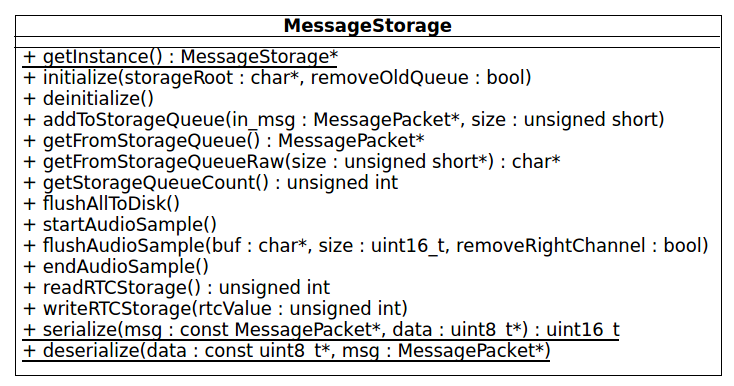
\includegraphics[width=0.7\textwidth]{Images/message_storage}
\caption{Class Diagram: MessageStorage}
\label{fig:class_message_storage}
\end{figure}

Our \textit{MessageStorage} class takes advantage of this and offers a simple enqueue-dequeue interface to the rest of the system. Aside from having the ability to flush all messages to SD when desired, the rest of the system does not actually know if elements in the message queue are stored in-memory or on-disk. MessageStorage maintains internal structures to keep track of each message in the queue, and where it is stored (memory or disk). While our current implementation relies on the flushAllToDisk function being externally called to save data to the SD card, it would be simple to implement a simple mechanism that checks of much memory is in use by the in-memory storage and flush this to disk to free up system memory.

Messages that will be stored on disk or in memory are serialized in the same manner as they are serialized when they are prepared for transmission over the wireless connection. Details of the message structure and the serialization process can be found in section \ref{sec:message_serialization}.

\begin{figure}[htb]
\centering
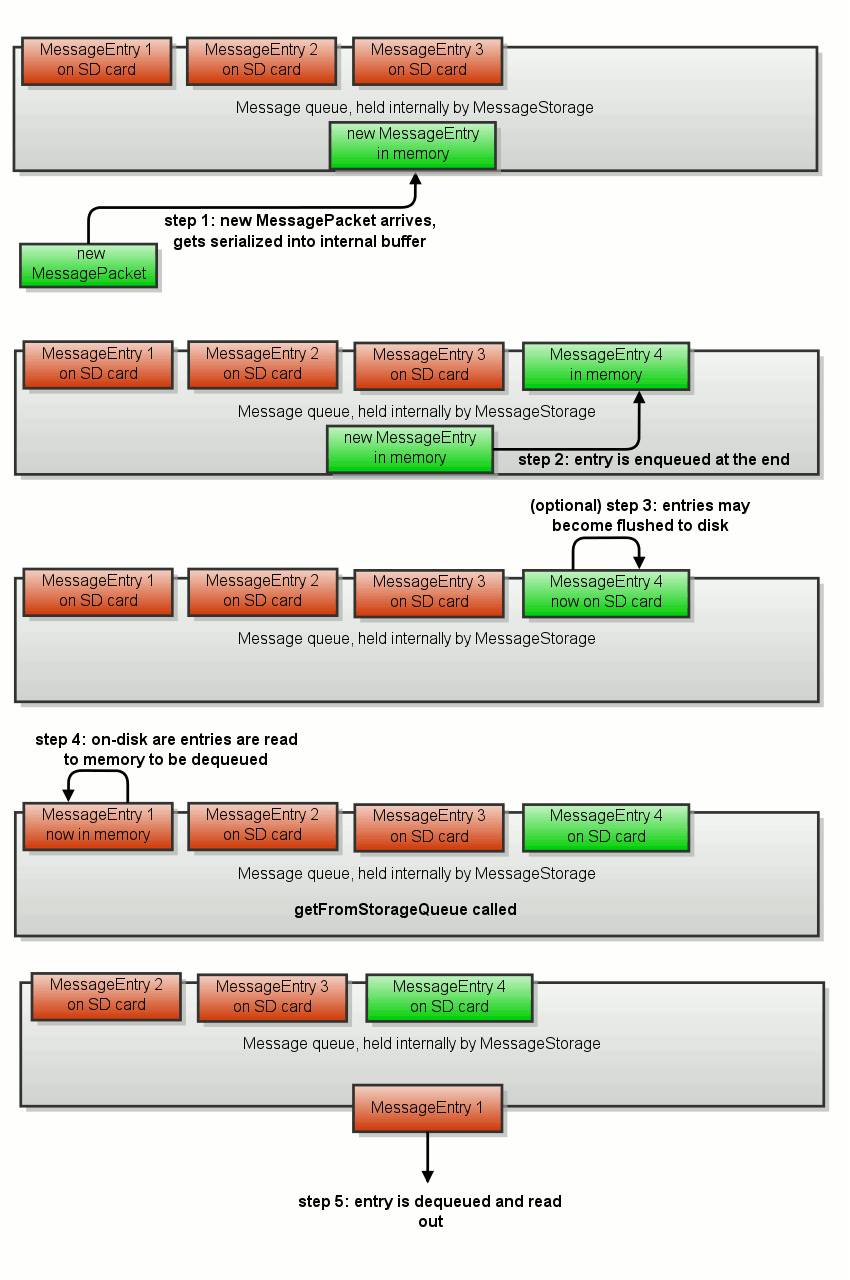
\includegraphics[width=0.9\textwidth]{Images/message_storage_lifecycle_fix}
\caption{ messages inside MessageStorage}
\label{fig:class_message_storage_dynamic}
\end{figure}

Figure \ref{fig:class_message_storage_dynamic} illustrates the lifetime of a message inside the MessageStorage class. The data is passed to MessageStore in the form of a MessagePacket pointer, which is first serialized into an internal dynamically allocated buffer and enqueued at the end of the message queue. If requested, this queue entry is flushed to disk and the allocated memory is freed. When the time comes to dequeue this entry for sending, the entry is first read back into memory if it was flushed to disk. The data in memory is then made available for sending via the ZigBee interface or otherwise processing the message data. Once the processing is complete, all resources held by the entry (files on disk or memory) can be freed or deleted.

If the system is rebooted, the class traverses the SD card storage directories to fill the queue with the unsent messages, and these become the first to be dequeued and sent to the base station.


\subsubsection{Automated Data Acquisition: DMA and Double Buffering}
Among the different on-chip peripherals included in the EFM32GG microcontroller is a DMA controller which allows for memory transfers without CPU intervention. 

\paragraph{Direct Memory Acess (DMA):}
\TODO{} DMA allows blocks of data to be moved between RAM and peripherals, thus freeing CPU resources and allowing longer periods of sleep, as well as offering stable high bandwidth memory transfers for operations like audio acquisition.
HW support: DMA engine
SW usage: setup, triggers, irq when done

\paragraph{Advantages:}
\TODO{} Direct Memory Access is a very valuable feature that allows for a better utilization of the system data bus and lower energy consumption.
why? decreases load on CPU and allows more sleep, guarantees better timings for time-critical/BW-critical operations - TODO Jose

\paragraph{Double-buffered DMA (Ping pong)}
\begin{figure}[htb]
\centering
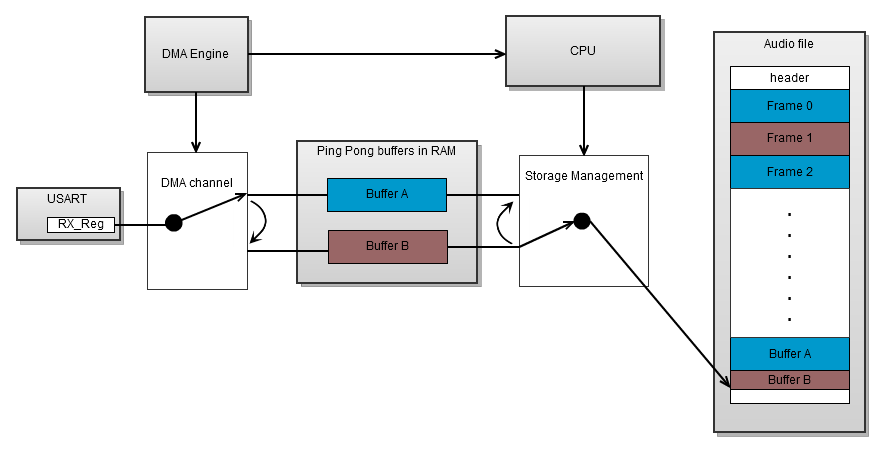
\includegraphics[width=\textwidth]{Images/ping_pong}
\caption{Ping Pong diagram}
\label{fig:ping_pong}
\end{figure}
\TODO{} PIng pong; insert \ref{fig:ping_pong} and explain it.


\section{Wireless Communications}
\label{sec:wireless_communication_software}

\subsection{XBee basics: Transparent vs. API}
The XBee firmware can operate in two modes, transparent and API. Transparent mode is the simplest way to use the XBee devices and it can be seen as a serial line replacement between two nodes. The problem with this mode is that it is not suited for complex network configurations. Every time a network parameter has to be changed (e.g. destination address) the devices have to enter a configuration mode which alone takes two seconds. In addition the mode is not suited for transmitting larger message frames. 

The second mode of operation is called API mode. This is a frame based approach, where all all data and command messages have to be packed into well defined frames where informations like destination are contained in the message header and device parameters can be changed on the fly. In addition this mode makes it possible to implement a more reliable data link, because successful transmission of each frame is acknowledged.

For these reasons the system uses the modules in API mode. This adds complexity to the implementation because it requires an intermediate layer for creating the frames according to the specifications, but the advantages we get from this mode outweigh the additional effort that has to be put into the implementation. 


\subsubsection*{libgebee}
Libgebee\footnote{\url{http://sourceforge.net/projects/libgbee}} is an open-source library written in C that provides a portable interface for accessing XBee devices. Its main task is creating XBee compatible frames, while hiding away low level procedures and base system dependent interactions with the serial port.

Because library has been written for the ZNet 2.5 XBee standard which has been replaced by the ZB standard over the last year it was necessary to update the library source code by adding newly introduced frame-types and updating existing ones to the new standard. These additions might flow back into the official repository if the author is interested in a cooperation.

The library also needed to be ported to the Energy Micro architecture before it could be used on the monitoring devices. Because the library aims at portability, it has a well defined interface between target system dependent functionality and the actual functionality of the library, which makes porting the library to a new architecture significantly easier. In our case, porting to the EFM32 architecture was almost trivial using the developed port/bus abstraction classes described in section \ref{sec:port_configuration} for the UART interface and the timekeeping class described in section \ref{sec:timekeeping} for operation timeouts.


\subsection{XBee Interface}
While the libgebee driver adds a nice layer of abstraction over the construction of API frames, it is not well suited for the direct use in an application with the complexity of the system we are building. Too many function calls are required to transmit or receive data and it would lead to a large amount of code repetition.  Furthermore our core application is written in C++ which allows for a higher level of abstraction.

\begin{figure}
\centering
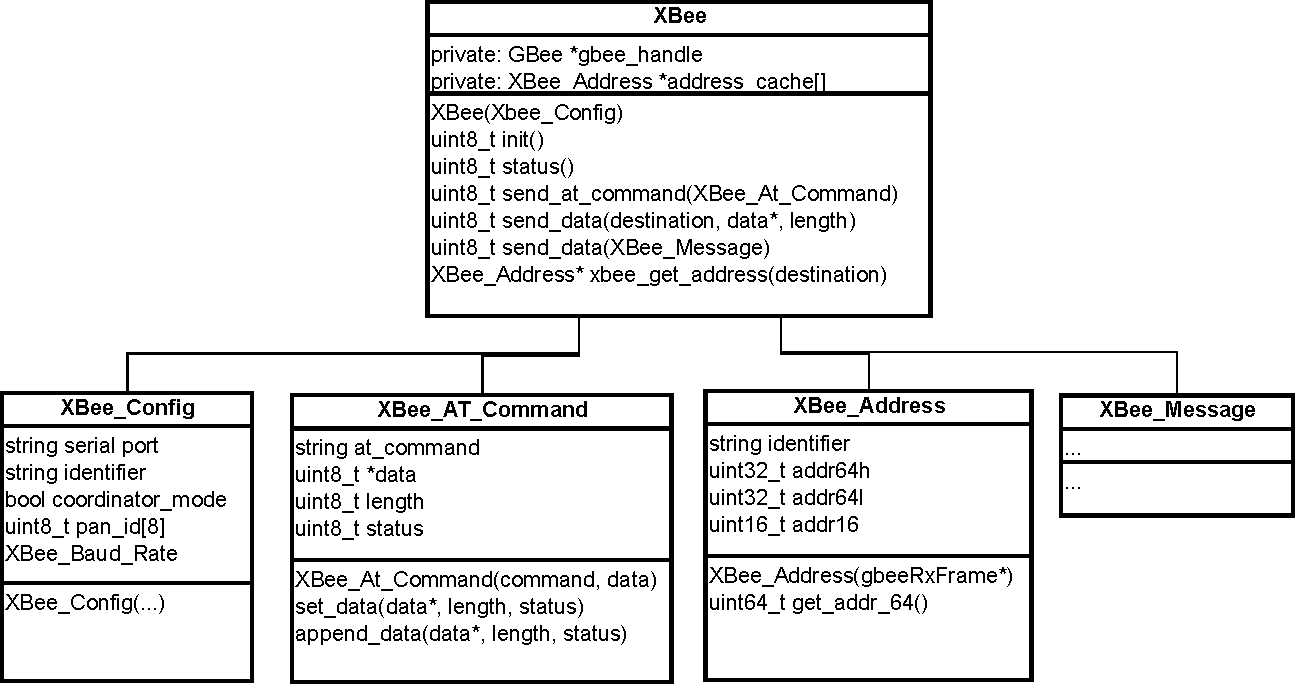
\includegraphics[width=\textwidth]{Images/xbee_interface}
\caption{Class diagram: XBee Interface}
\label{fig:xbee_interface}
\end{figure}

A C++ wrapper and a number of utility classes were developed to simplify data transmission and control of XBee devices (from the viewpoint of the core application). Figure \ref{fig:xbee_interface} shows the public interface functions of this wrapper and the utility classes will be discussed in the following sections

\subsection{Message handling}
The size of data frames that can be transmitted over ZigBee networks in one transmission is limited to a payload size of 84 Bytes. Our system needs to be capable of sending and receiving messages that exceed this size limit by multiple factors. For this purpose a XBee\_Message class was implemented that takes care of chopping arbitrary sized messages into frame sized pieces and re-assembling messages from received frames. 

\subsubsection{XBee\_Message}
\begin{figure}
\centering
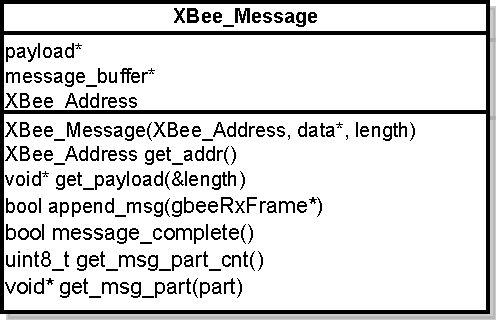
\includegraphics[width=0.5\textwidth]{Images/xbee_message}
\caption{Class diagram: XBee Message}
\label{fig:xbee_message}
\end{figure}

The XBee\_Message class expects a pointer to the data that should be packed into the message and the size of the data field. During instantiation the data is copied into a object internal buffer and the object takes over the responsibility for handling the allocated memory. 

The XBee interface uses objects of this class internally for message handling and also accepts objects of this kind as parameters for the send function. When data is received over the ZigBee network, the append\_msg function of this class is used to reconstruct the messages consisting of multiple parts before passing a handle to a complete message object to the user.

The XBee\_Message class is aimed at handling arbitrary data of arbitrary size and does neither know nor care about the type of data it contains. It treats all data in exactly the same way. The definition of the data that allows us to give a meaning to it is done independently.

\subsubsection{Message Types}
\label{sec:message_types}
The previous paragraph explained how the XBee\_Message class is used to transfer arbitrary data between network nodes. This paragraph deals with the way in which meaning is added to this data.

We use an inheritance based approach to define message types. Inheritance is particularly suited for this case as we can group messages into categories that have many common fields and only limited need for specialization.

\begin{figure}
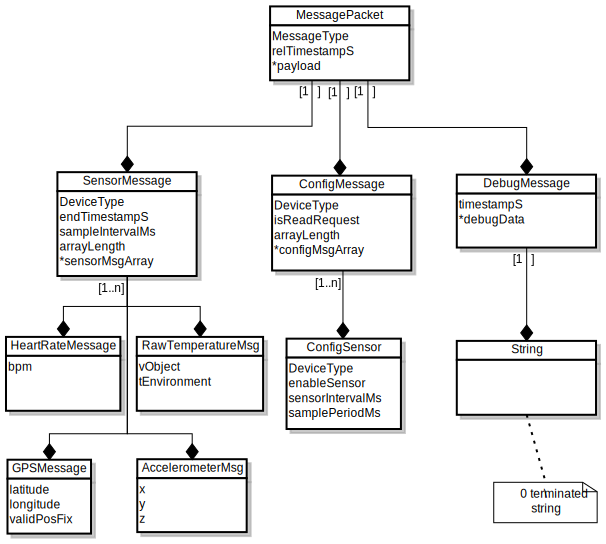
\includegraphics[width=\textwidth]{Images/message_types}
\caption{Class diagram: Message Types}
\label{fig:msg_types}
\end{figure}

This is implemented with structures instead of classes because structures guarantee that members are stored sequentially in memory which makes the job of serializing and de-serializing the messages for transmission purposes a lot easier.

The design of the message type classes allows to pack an array of multiple measurements (from the same sensor) into one message, which can help to increase the data throughput by improving to data to overhead ratio.

\subsubsection{Message de-/serialization}
\label{sec:message_serialization}
\begin{figure}
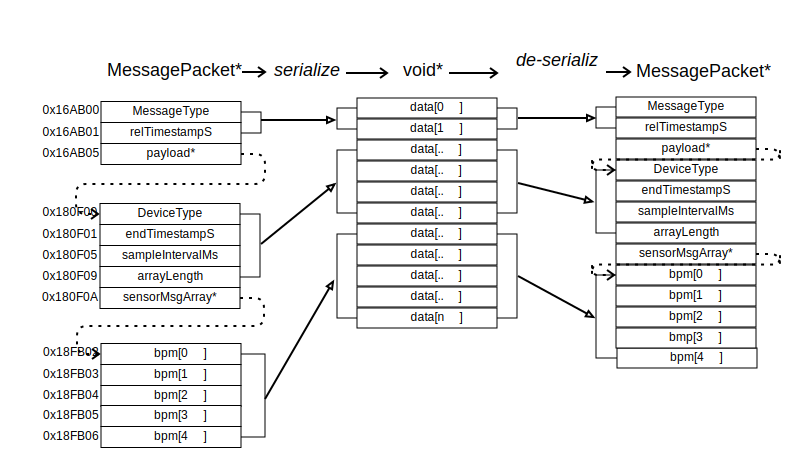
\includegraphics[width=\textwidth]{Images/msg_serialization}
\caption{Message serialization}
\label{fig:msg_serialization}
\end{figure}

The inheritance based message type data structures make extensive use of references, which is why they cannot be used for transmission as they are, but have to be serialized first. The process of serialization follows the references and copies all data of the message into a continuous memory area that can be transmitted across the ZigBee network, and deserialized into a message object on the other side. Figure \ref{fig:msg_serialization} depicts the steps involved in the process.

Message de-/serialization is implemented by two free-standing functions. The one that performs serialization expect a MessagePacket (see \ref{sec:message_types}) and a pointer to pre-allocated memory as arguments and copies the values from the MessagePacket into the continous memory. The deserialize function performs the inverse of this operation, and returns a MessagePacket that is an exact copy of the source MessagePacket, except for the destinations of the pointer members.

\subsubsection{Timestamps - relative and absolute timekeeping}
The timekeeping of the system is based on a the Unix style Real Time Clock (RTC), with the peculiarity that the monitoring devices do not count absolute time but time relative to the moment when they were first switched on. This decision is based on the fact that we cannot guarantee that the monitoring devices are able sync their internal RTC to the RTC of the base station when they are switched on (base station not in range, no GPS signal) which might lead to artifacts in the measurement data.

\begin{center}
\begin{math}
T_{abs} = RTC_{abs}- (T_{transmission} - T_{measurement})
\end{math}
\end{center}

To calculate the absolute time when a measurement was taken, the messages contain two relative timestamps - one that shows when the measurement was taken, and one that shows when the measurement was transmitted. The absolute time is calculated on the base station, right before the message is stored in the database.


\section{Base station software}
There are two independent software modules running on the base station software that use different Inter-process communication methods (IPC) to cooperate with each other. The receive and store module (R\&S) is responsible for the communication with the monitoring devices and storing received data into a database. The data presentation module on the other hand provides a graphical user interface (GUI) for the collected data and allows the user to configure the base station and the monitoring devices connected to the network.

The decision to divide the base station software into two independent parts was based on the fact that is is possible to create a very clear and well defined interface between the two modules. This allows us to develop the parts independently and use different programming languages that are best suited for the task. It also makes it possible to modify or replace the data presentation module without the need to adapt the rest of the system.

This is especially important in the case of the data presentation module, because we cannot foresee how the collected data is going to be used, and what is the optimal way of presenting the data to the user. In addition to that, the task of analysing and presenting the data was assigned to our sixth team member during the planning phase of the project, and had to be taken over by the rest of the team. For this reason we could not allocate as many man-hours to the presentation module as we would have liked, as it is a non-critical part of the system.

\subsection{Inter-process communication}
\subsubsection*{Database}
A file based sql database (sqlite3) is used to share the collected data and information about network status and node configuration between the two modules. The direction of communication is one-sided. The receive and store module writes to the database and when the user accesses the web interface the data presentation module extracts the requested information from the database. It can be seen as a passive way of communication as the one side who writes to the database does not care about the other side.


\subsubsection*{Message queues}
POSIX message queues are used to implement reactive communication between the processes, e.g. if the user requested a change of configuration in the web interface. The R\&S module will check the message queue periodically and react to them as promptly as possible. In case of messages that affect the base station the commands are executed almost immediately, in case of messages that concern monitoring devices, the messages are queued until the device connects to the base station, and the message can be dispatched.

\subsection{Receive and store module}
The receive and store module sets up and controls the  ZigBee network and provides measurement data storage facilities in a sqlite3 database. It implements a simple state machine, waiting for incoming messages over the ZigBee network or the IPC message queue.

When there is incoming data from the ZigBee network, the module enters the receive state and tries to receive an XBee\_Message. When a complete XBee\_Message is successfully received, the message content is deserialized and stored into the database. When there’s not pending data left, the message queue is checked for messages destined for the node that just transmitted data. In case there are pending messages, they are dispatched, else the module goes back into the idle state.

When there is incoming data over the message queue, the module checks if the request can be handled locally in which case it is executed immediately. If the request is directed at a monitoring device, the R\&S has to defer dispatching the request until the next time the destined monitoring device connects to the base station. The reasons why the base station has to wait for the monitoring devices to open up a communication channel were explained in section
\ref{sec:wireless_connection}

\subsection{Data presentation module}
The data presentation module is written in Python and uses a lightweight Python web framework (flask\footnote{\url{http://flask.pocoo.org}}) to generate the web interface dynamically. 

The use of a dynamic programming language to generate the content that the user can see dynamically allows us to build a dynamic webinterface with a backend that’s communicating with the controller software. 

\subsubsection*{Web Interface}
The framework strictly divides display and logic parts of the website. The dynamic content of the pages is generated on the fly with the whole functionality of Python. This has the advantage that the menus of the website automatically get extended with sub-menus if a new monitoring device connects to the base station. 

\begin{figure}
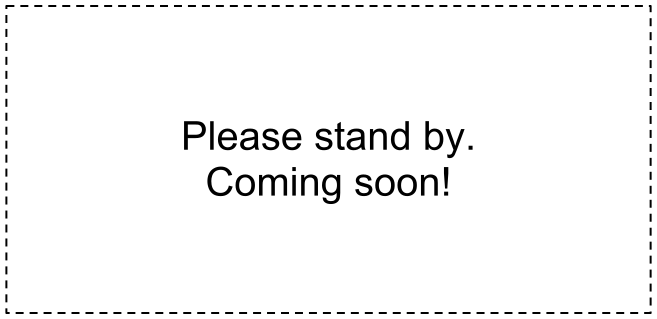
\includegraphics[width=\textwidth]{Images/dummy}
\caption{Web Interface}
\label{fig:web_interface}
\end{figure}

The sensor data is currently displayed in dynamically generated static html tables. This allows a good quick overview over the collected data, but is suboptimal to analyze the data in more detail. In future versions this could be improved by using Ajax to display the tables, to offer better access to the collected data.









